\section{Nonlinear SDE experiments}\label{app:sec:nonlinear-sde}

In this section, we provide additional details on our three nonlinear SDE experiments: the stochastic Lorenz attractor (\Cref{app:subsec:lorenz}), rotifer-algae predator-prey dynamics (\Cref{app:subsec:predator-prey}), and reduced order models for fluid dynamics (\Cref{app:subsec:rom}).

For all experiments we use a Gaussian posterior approximation $q(\mbx, t) = \cN(\mbm(t), \mbS(t))$ with dense $\mbS \in \bbR^{K \times K}$.
We also use the Adam optimizer \cite{kingma2014adam} with exponential learning rate decay. 
We run experiments on an NVIDIA A100 or H100 GPU.

\subsection{Noisy Lorenz attractor}\label{app:subsec:lorenz}

\begin{figure*}[!t]
  \centering
  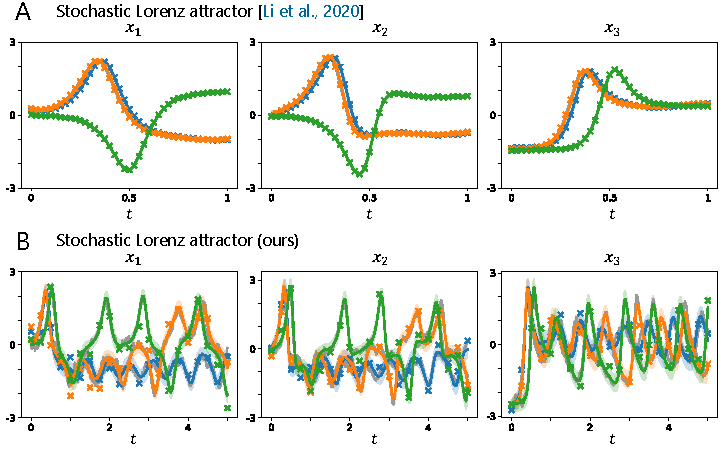
\includegraphics[width=\textwidth]{figs/fig5-lorenz-compare.pdf}
  \caption{
    Visualization of three samples of the stochastic Lorenz attractor dataset from \citet{li2020scalable} (\textbf{A}) and this paper (\textbf{B}).
    Grey curves represent the true latent trajectory and colored $\times$ represent regularly-spaced observations.
    Colored curves represent the posterior mean and shading represents $\pm2$ posterior standard deviations obtained from the iterated extended Rauch-Tung-Striebel smoother (\citet[][Chapter 13.3]{sarkka2023bayesian}). The Bayesian posterior in \citet{li2020scalable} collapses to the true latent trajectory, whereas our dataset displays non-trivial posterior variance.
  }
  \label{fig:lorenz-compare}
\end{figure*}


\paragraph{Data generation.}
We generate a dataset consisting of $1024$ training samples and $2048$ test samples according to the $3$-dimensional Lorenz attractor dynamics
\begin{equation}\label{app:eqn:lorenz}
d \mbx(t) = \begin{pmatrix} \alpha(\mbx_2(t) - \mbx_1(t))\\
\mbx_1(t)(\rho - \mbx_3(t)) - \mbx_2(t)\\
\mbx_1(t)\mbx_2(t) - \beta \mbx_3(t)
\end{pmatrix} dt + \sigma d\mbw(t), \quad \mbx(0) \sim \cN(\mb{0}, \bbI_3), \quad 0 \leq t \leq T
\end{equation}
where $(\alpha, \rho, \beta) = (10, 28, 8/3)$ and $\sigma > 0$ is the diffusion scaling. 
We do so using the Euler--Maruyama sampler with discretization $10^{-3}$. 

Following \citet{li2020scalable}, we make observations of the latent state every $\Delta t$ according to $\mbC_{\mathrm{true}} \mbx(t) + \mbd_{\mathrm{true}} + \mbepsilon(t)$, $\mbepsilon(t) \sim \cN(\mb{0}, \eta^2 \bbI_3)$, where $\mbC_{\mathrm{true}} = \mathrm{diag}(\mbs^{-1})$ and $\mbd_{\mathrm{true}} = - \mbm \odot \mbs^{-1}$; $\mbm, \mbs \in \bbR^3$ represent the empirical mean and standard deviation of the training trajectories, respectively, along each dimension and pooled across time. 
$\eta > 0$ is the observation standard deviation.

In the standard stochastic Lorenz attractor, the authors choose $T = 1$ and parameters $(\Delta t, \sigma, \eta) = (2.5 \cdot 10^{-2}, 1.5 \cdot 10^{-1}, 10^{-2})$. 
In the observation coordinates, the effective diffusion coefficient is $\sigma \mbs^{-1} \approx (1.7 \cdot 10^{-2}, 1.3 \cdot 10^{-2}, 9.8 \cdot 10^{-3})$, which is exceedingly small relative to the scale on which the latents evolve. 
As a result of the small process noise, frequent observations, and small measurement noise, we observe that the posterior collapses to the true latent trajectory (\Cref{fig:lorenz-compare}). 
Methods that differ substantially in how they represent or sample posterior uncertainty are therefore indistinguishable on this benchmark. 

We instead simulate the latents over a long interval $T = 5$ with larger process noise $\sigma = 5$, less frequent observations $\Delta t = 2.5 \cdot 10^{-1}$, and larger measurement noise $\eta = 0.3$. 
In this case, the effective diffusion coefficient in the observation space is $\sigma \mbs^{-1} \approx (6.0 \cdot 10^{-1}, 5.2 \cdot 10^{-1}, 5.2 \cdot 10^{-1})$. 
We find that this setting leads both to more interesting latent trajectories (frequent switching between lobes of the attractor, which is not demonstrated in the original dataset; \Cref{fig:lorenz-samples}A) and nontrivial posterior uncertainty (\Cref{fig:lorenz-compare}). 

\paragraph{Generative model.}
Consistent with prior work, we learn a $K = 4$ dimensional latent dynamical system representing the Lorenz attractor. 
The prior initial state is modeled as Gaussian $\cN(\mbmu_0, \mbV_0)$, $\mbmu_0 \in \bbR^4$, $\mbV_0 \in \bbR^{4 \times 4}$; the prior drift function \cref{eqn:prior_sde} is a neural network; and the observation model is linear and Gaussian $\cN(\mby(t) | \mbC \mbx(t) + \mbd, \sigma_{\mathrm{obs}}^2 \bbI)$, $\mbC \in \bbR^{3 \times 4}$, $\mbd \in \bbR^3$, $\sigma_{\mathrm{obs}} > 0$.
We learn the parameters of the prior SDE and observation model jointly with those of the posterior.

\paragraph{Baselines.}
We compare Helmholtz-SDE to two simulation-free VI algorithms, ARCTA \cite{course2023amortized} and SDE-Matching \cite{bartosh2025sde}, as well as two simulation-based VI algorithms, SING \cite{hu2025sing} and Latent SDE \cite{li2020scalable}.
Note that `ARCTA' simply describes an amortization strategy for SVISE \cite{course2023state}. In particular, the variational drift, the symmetric gauge, remains the same.

We aim to reproduce the Lorenz attractor experimental setup as faithfully as possible from the original papers, with our modified data generation procedure. 
Among these algorithms, there are two noteworthy differences: 
(1) SDE Matching \cite{bartosh2025sde} and Latent SDE \cite{li2020scalable} support state-dependent diffusion coefficients; 
and (2) SING does not support an amortized posterior approximation. 
For SING, we discretize the posterior on a grid of size $10^{-3}$ and use mini-batches of $500$ trials; mini-batching is necessary since the posteriors for all $1024$ trials cannot fit simultaneously into memory (on an 80 GB GPU).
We performed a small sweep over the SING mini-batch size and grid size.

For Helmholtz-SDE, we adopt the same amortization strategy employed by SDE-Matching \cite{bartosh2025sde} and Latent SDE \cite{li2020scalable} wherein for each trial, the sequence of observations is encoded by a GRU to produce an embedding. 
This embedding is then passed through an MLP to represent the posterior at each time. 
This strategy shares the posterior both across trials and across time.

We used the ARCTA (\url{https://github.com/coursekevin/arlatentsde}), SDE-Matching (\url{https://github.com/GrigoryBartosh/sde_matching}), SING (\url{https://github.com/lindermanlab/sing}), and Latent SDE (\url{https://github.com/google-research/torchsde}) codebases, with modifications as described below.

\begin{itemize}
    \item \textbf{Helmholtz-SDE}:
    \begin{itemize}
        \item \texttt{latent\_dim = 4}, \texttt{obs\_dim = 3},  \texttt{time\_dim = 1}, \texttt{hidden\_dim = 100}
        \item 
        Prior drift:\\
        \texttt{(latent\_dim) $\to$ Linear(latent\_dim, hidden\_dim) $\to$ Softplus $\to$ Linear(hidden\_dim, latent\_dim) $\to$ (latent\_dim)}
        \item Posterior encoder:\\ \texttt{(n\_obs, obs\_dim) $\to$ GRU $\to$ (n\_obs + 1, hidden\_dim)}
        \item Posterior MLP:\\ 
        for a specified time, aggregate embeddings from encoder using softmax, \\
        \texttt{(n\_obs + 1, hidden\_dim), (time\_dim) $\to$ softmax $\to$  (hidden\_dim)}\\
        then map to posterior at that time\\
        \texttt{(hidden\_dim + time\_dim) $\to$ Linear(hidden\_dim + time\_dim, hidden\_dim) $\to$ SiLU  $\to$ Linear(hidden\_dim, hidden\_dim) $\to$ SiLU $\to$ Linear(hidden\_dim, output\_dim) $\to$ (output\_dim)}\\
        where \texttt{output\_dim} is \texttt{latent\_dim} (mean) + \texttt{latent\_dim $\cdot$ (latent\_dim + 1) / 2} (covariance)
        \item Diffusion network: fixed $\bbI_{\texttt{latent\_dim}}$
        \item Helmholtz correction: linear approximation $\ell = 1$, computed using the Stein estimand with $N_{\mathrm{mc}} = 1$
        \item Observation model: fixed covariance $\sigma_{\mathrm{obs}}^2 = \eta^2$, learned $\mbC$, $\mbd$
        \item LR: $10^{-3}$ (constant)
        \item Gradient clipping: $5.0$
        \item Iterations: $3 \cdot 10^4$
        \item Number MC samples (per iteration): $N_{\mathrm{time}} = 1$ sample over $[0, T]$ to estimate each of the KL and reconstruction loss, per trial
    \end{itemize}
    \item \textbf{SDE Matching}:
    \begin{itemize}
        \item \texttt{latent\_dim = 4}, \texttt{obs\_dim = 3},  \texttt{time\_dim = 1}, \texttt{hidden\_dim = 100}
        \item 
        Prior drift:\\
        \texttt{(latent\_dim) $\to$ Linear(latent\_dim, hidden\_dim) $\to$ Softplus $\to$ Linear(hidden\_dim, latent\_dim) $\to$ (latent\_dim)}
        \item Posterior encoder:\\ \texttt{(n\_obs, obs\_dim) $\to$ GRU $\to$ (n\_obs + 1, hidden\_dim)}
        \item Posterior MLP:\\ 
        for a specified time, aggregate embeddings from encoder using softmax, \\
        \texttt{(n\_obs + 1, hidden\_dim), (time\_dim) $\to$ softmax $\to$  (hidden\_dim)}\\
        then map to posterior at that time\\
        \texttt{(hidden\_dim + time\_dim) $\to$ Linear(hidden\_dim + time\_dim, hidden\_dim) $\to$ SiLU  $\to$ Linear(hidden\_dim, hidden\_dim) $\to$ SiLU $\to$ Linear(hidden\_dim, output\_dim) $\to$ (output\_dim)}\\
        where \texttt{output\_dim} is \texttt{latent\_dim} (mean) + \texttt{latent\_dim $\cdot$ (latent\_dim + 1) / 2} (covariance)
        \item Diffusion network:\\ 
        state-dependent, diagonal diffusion coefficient; the input to each diagonal entry is a single hidden dimension\\
        \texttt{latent\_dim $\times$ [(1) $\to$ Linear(1, hidden\_dim) $\to$ Softplus $\to$ Linear(hidden\_dim, 1) $\to$ Sigmoid $\to$ (1)]}
        \item Observation model: fixed covariance $\sigma_{\mathrm{obs}}^2 = \eta^2$, learned $\mbC$, $\mbd$
        \item LR: $10^{-3}$ (constant)
        \item Gradient clipping: $5.0$
        \item Iterations: $3 \cdot 10^4$
        \item Number MC samples (per iteration): $N_{\mathrm{time}} = 1$ sample over $[0, T]$ to estimate each of the KL and reconstruction loss, per trial
    \end{itemize}
    \item \textbf{ARCTA}:
    We found that the Gaussian process parameterization of the posterior described by \citet{course2023amortized} (see Appendix D therein) led to poor empirical performance. This is because, at a high level, the posterior defines the mean and covariance at each time as a linear combination of means and covariances at observation times.
    Since in our setting the observations occur sparsely in time, interpolating in the space of means and covariances directly is inappropriate. 
    Instead, we adopt the posterior parameterization from SDE Matching, wherein interpolation occurs in the embedding space \cite{bartosh2025sde}.

    Moreover, \citet{course2023amortized} propose chunking the full time series of observations into non-overlapping windows. For each observation within a given window, they produce an embedding using a specified number of future observations, and then they aggregate embeddings within the window. We find that choosing window size and a number of observations smaller than the full time series degrades performance. For this reason, we consider a window equal to the full time series and allow each embedding to depend on all future observations.   
   
    \begin{itemize}
        \item \texttt{latent\_dim = 4}, \texttt{obs\_dim = 3},  \texttt{time\_dim = 1}, \texttt{hidden\_dim = 100}
        \item 
        Prior drift:\\
        \texttt{(latent\_dim) $\to$ Linear(latent\_dim, hidden\_dim) $\to$ Softplus $\to$ Linear(hidden\_dim, latent\_dim) $\to$ (latent\_dim)}
        \item Posterior encoder:\\ \texttt{(n\_obs, obs\_dim) $\to$ GRU $\to$ (n\_obs, hidden\_dim)}
        \item Posterior MLP:\\ 
        for a specified time, aggregate embeddings from encoder using softmax, \\
        \texttt{(n\_obs, hidden\_dim), (time\_dim) $\to$ softmax $\to$  (hidden\_dim)}\\
        then map to posterior at that time\\
        \texttt{(hidden\_dim + time\_dim) $\to$ Linear(hidden\_dim + time\_dim, hidden\_dim) $\to$ SiLU  $\to$ Linear(hidden\_dim, hidden\_dim) $\to$ SiLU $\to$ Linear(hidden\_dim, output\_dim) $\to$ (output\_dim)}\\
        where \texttt{output\_dim} is \texttt{latent\_dim} (mean) + \texttt{latent\_dim $\cdot$ (latent\_dim + 1) / 2} (covariance)
        \item Diffusion network: fixed $\bbI_{\texttt{latent\_dim}}$
        \item Observation model: fixed covariance $\sigma_{\mathrm{obs}}^2 = \eta^2$, learned $\mbC$, $\mbd$
        \item LR: $10^{-3}$ (constant)
        \item Gradient clipping: $5.0$
        \item Iterations: $3 \cdot 10^4$ 
        \item Number MC samples (per iteration): $1$ sample over $[0, T]$ to estimate the KL, per trial; use full set of per-trial observations at each step to estimate reconstruction loss (for consistency with ARCTA window algorithm)
    \end{itemize}
    \item \textbf{SING}:
    \begin{itemize}
        \item \texttt{latent\_dim = 4}, \texttt{obs\_dim = 3},  \texttt{hidden\_dim = 100},
        \texttt{grid\_size = $5 \cdot 10^3$ + 1}
        \item 
        Prior drift:\\
        \texttt{(latent\_dim) $\to$ Linear(latent\_dim, hidden\_dim) $\to$ Softplus $\to$ Linear(hidden\_dim, latent\_dim) $\to$ (latent\_dim)}
        \item Posterior (non-amortized): tensors of shape \texttt{(grid\_size, latent\_dim)} (mean), \texttt{(grid\_size, latent\_dim, latent\_dim)} (covariance), \texttt{(grid\_size - 1, latent\_dim, latent\_dim)} (cross-covariance)
        \item Diffusion network: fixed $\bbI_{\texttt{latent\_dim}}$
        \item Observation model: fixed covariance $\sigma_{\mathrm{obs}}^2 = \eta^2$, learned $\mbC$, $\mbd$
        \item Mini-batch size: $500$
        \item LR: 
        \begin{itemize}
            \item SING stepsize (i.e., natural gradient update): $10^{-3}$ to $10^{-2}$ on log-linear scale for first $10$ iterations, constant after
            \item M-step stepsize: $5 \cdot 10^{-3}$ (Adam)
        \end{itemize}
        \item Gradient clipping: $5.0$
        \item Iterations: for each iteration perform 1 SING step, 1 M-step gradient update; $10^4$ total iterations
        \item Number MC samples (per iteration): $1$ sample to compute expectations under the prior
    \end{itemize}
    \item \textbf{Latent SDE}:
    \begin{itemize}
        \item \texttt{latent\_dim = 4}, \texttt{obs\_dim = 3},  \texttt{time\_dim = 1}, \texttt{hidden\_dim = 128}, \texttt{embedding\_dim = 64}
        \item 
        Prior drift:\\
        \texttt{(latent\_dim) $\to$ Linear(latent\_dim, hidden\_dim) $\to$ Softplus $\to$ Linear(hidden\_dim, hidden\_dim) $\to$ Softplus $\to$ Linear(hidden\_dim, latent\_dim) $\to$ (latent\_dim)}
        \item Posterior encoder:\\ \texttt{(n\_obs, obs\_dim) $\to$ reverse $\to$ GRU $\to$ reverse $\to$ (n\_obs, hidden\_dim) $\to$ Linear(hidden\_dim, embedding\_dim) $\to$ (embedding\_dim)}
        \item Posterior drift network:\\ 
        for a specified latent state, use embedding to produce drift\\
        \texttt{(latent\_dim + embedding\_dim) $\to$ Linear(latent\_dim + embedding\_dim, hidden\_dim) $\to$ Softplus $\to$ Linear(hidden\_dim, hidden\_dim) $\to$ Softplus $\to$ Linear(hidden\_dim, latent\_dim) $\to$ (latent\_dim)}
        \item Posterior initial distribution:\\
        use embedding to produce distribution (Gaussian) over initial latent state\\
        \texttt{(embedding\_dim) $\to$ Linear(embedding\_dim, latent\_dim + latent\_dim) $\to$ (latent\_dim + latent\_dim)}\\
        first \texttt{latent\_dim} outputs represent mean, second \texttt{latent\_dim} outputs represent log standard deviation
        \item Diffusion network:\\ 
        state-dependent, diagonal diffusion coefficient; the input to each diagonal entry is a single hidden dimension\\
        \texttt{latent\_dim $\times$ [(1) $\to$ Linear(1, hidden\_dim) $\to$ Softplus $\to$ Linear(hidden\_dim, 1) $\to$ Sigmoid $\to$ (1)]}
        \item Observation model: fixed covariance $\sigma_{\mathrm{obs}}^2 = \eta^2$, learned $\mbC$, $\mbd$
        \item Training discretization: $10^{-2}$ (for posterior sampling)
        \item LR: initial $10^{-3}$, final $10^{-4}$ (exponential LR decay)
        \item Gradient clipping: None
        \item Iterations: $3 \cdot 10^4$
        \item KL annealing iterations: $10^3$ 
        \item Number MC samples (per iteration): $1$ path simulated from the posterior per trial

    \end{itemize}
\end{itemize}

\paragraph{Metrics.}\leavevmode\\

We evaluate the fidelity of the posterior and prior dynamics according to five metrics, which we explain below.

\textbf{nELBO.} Average per-trial negative ELBO (the variational objective). Smaller values are better but do not imply better posterior recovery or learning.

\textbf{Posterior inference.}
To evaluate posterior quality, we use the log likelihood of the true latents  under the posterior distribution averaged over time $T$ and trials $M$, calculated as 
\begin{equation}\label{app:eqn:predictive-prob}
   \frac{1}{TM} \sum_{m, t} \log 
\bar{q}(\mby^{(m)}(t), t).
\end{equation}
$\bar{q}(\mby, t)$ represents the posterior predictive density of  $\bar{\mby}(t) = \mbC \mbx(t) + \mbd + \mbepsilon(t), \ \mbepsilon(t) \sim \cN(\mb{0}, \mbR)$ and $\mby(t) = \mbC \mbx(t) + \mbd$ is the true latent at time $t$, passed through the output mapping. 
We exclude training observations from the sum \cref{app:eqn:predictive-prob}.


For all cases except Latent SDE \cite{li2020scalable}, $q(\mbx, t) = \cN(\mbm(t), \mbS(t))$ is Gaussian, in which case  the posterior predictive distribution admits a closed form $\bar{q}(\mby, t) = \cN(\mbC \mbm(t) + \mbd, \mbC \mbS(t) \mbC^\top + \mbR)$.
For Latent SDE, we estimate $\bar{q}(\mby^{(m)}(t), t)$ by drawing $N_{\mathrm{density}} = 64$ samples $\mbx^{(k)}(t) \sim q(\mbx, t)$, computing $\bar{\mby}^{(k)}(t) =  \mbC \mbx^{(k)}(t) + \mbd$, and then evaluating
\begin{equation}\label{app:eqn:latent-sde-estimate}
    \frac{1}{TM} \sum_{m, t} \log \left(\frac{1}{N_{\mathrm{density}}} \sum_k \cN(\mby | \bar{\mby}^{(k)}(t), \mbR) \right).
\end{equation}
Note that \cref{app:eqn:latent-sde-estimate} is a sensible approximation to \cref{app:eqn:predictive-prob} since
{\small
\begin{equation*}
\begin{aligned}
    \bar{q}(\mby, t) &= \int q(\mbx, t) \cN(\mby | \mbC \mbx + \mbd, \mbR) d \mbx
    = \bbE_{q(\mbx, t)}[\cN(\mby | \mbC \mbx + \mbd, \mbR)] \approx \frac{1}{N_{\mathrm{density}}} \sum \cN(\mby | \bar{\mby}^{(k)}(t), \mbR).
\end{aligned}
\end{equation*}
}

\textbf{Prior learning.}
For evaluating the learned prior dynamics, we draw $2048$ samples from the learned prior, starting from $q(\mbx, 0)$ and simulated using Euler--Maruyama with discretization $10^{-3}$. 
We evaluate the learned output mapping at these samples, from which we compute the following metrics:
\begin{enumerate}[label=(\roman*)]
    \item \textbf{One-time symmetric KL divergence}: symmetric KL divergence at each time in $[0, T]$, averaged over times. 
    For samples from two distributions $p$ and $q$, we estimate the KL distance $\KL{p}{q}$ by fitting two Gaussian kernel density estimates and computing a Monte Carlo average.
    
    We do so using the following procedure, which mirrors that of \citet{kiyohara2025neural}:
    \begin{enumerate}
        \item Using 5-fold CV, select the KDE bandwidth for $q$; fit the density estimate (on all samples) using the chosen bandwidth.
        \item Split the samples from $p$ into $10$ folds. Holding out a single fold at a time, repeat the following subprocedure:
        \begin{enumerate}
            \item Choose the kernel bandwidth for $p$ using 5-fold CV; fit the density estimate (on all training folds) using the chosen bandwidth.
            \item Compute a Monte Carlo estimate of the KL divergence using the held-out fold.
        \end{enumerate}
    \end{enumerate}
    Importantly, the outer CV step for samples from $p$ ensures that the negative entropy is not systematically downward biased.
    
    \item \textbf{Global autocorrelation error}: Using the samples from learned prior and true prior, we estimate the correlation matrix at lag $0 \leq \tau \leq T$, $\mathrm{Corr}(\mbx(t), \mbx(t + \tau))$, for all $t$ such that $t, t + \tau$ lie on the sampling grid. 
    At each such time, we compute the squared Frobenius norm difference between the two correlation matrices and average over all valid times. We repeat this procedure for all lags $\tau$ on a linear grid of $[0, 2]$ with spacing $5 \cdot 10^{-2}$, and we average over these lags.
    Finally, we normalize by the total number of entries in the correlation matrix ($3 \times 3 = 9$) and take the square root of the result.
\end{enumerate}

\paragraph{Ablation of $q$-divergence-free correction.}
\begin{figure*}[h]
  \centering
  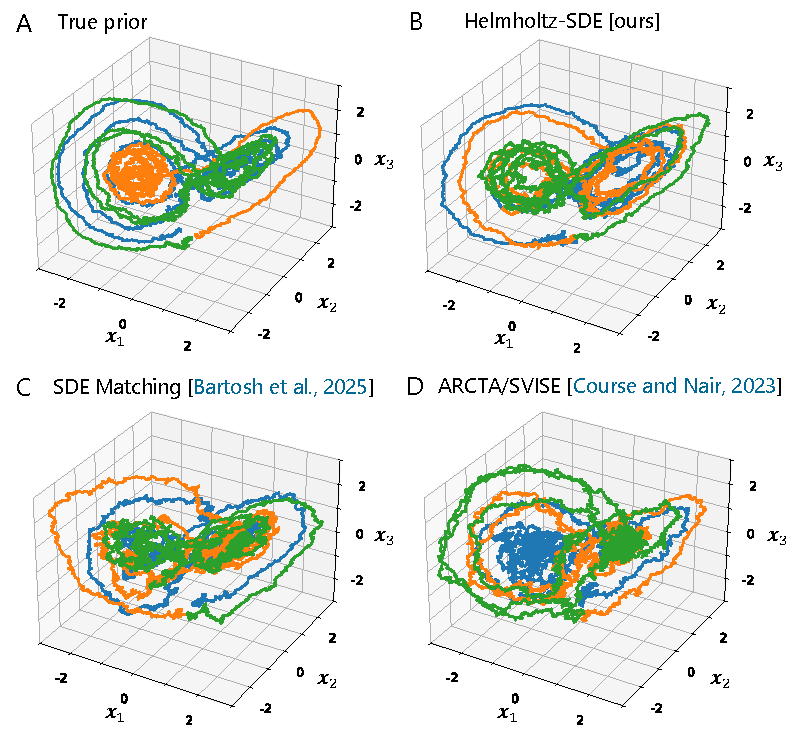
\includegraphics[width=0.9\textwidth]{figs/fig6-lorenz-samples.pdf}
  \caption{
   Three random samples from the 
   true prior (\textbf{A}),
   the prior learned by Helmholtz-SDE (\textbf{B}),
   SDE Matching (\textbf{C}),
   and ARCTA/SVISE (\textbf{D}).
   Helmholtz-SDE more faithfully learns the dynamics, particularly the outward spiral dynamics within each lobe of the attractor. 
  }\label{fig:lorenz-samples}
\end{figure*}

We report ablations over the $q$-divergence-free correction used by Helmholtz-SDE. 
In \Cref{tab:lorenz-nelbo}, we report the negative ELBO for polynomial degrees $\ell \in \{1, 2, 3\}$ and for different estimators of the polynomial divergence-free correction.
For all estimators, we evaluate the final negative ELBO using $N_{\mathrm{quad}} = 6$ quadrature points per dimension (i.e., the estimators differ during training but not evaluation).
$\kappa$ denotes the degree of the Stein estimand \cref{app:eq:stein-estimator}; when $\kappa$ is smaller than the polynomial degree $\ell$, we take derivatives of the largest entries of $\mbalpha$.

In general, we observe that the Stein estimand \cref{app:eq:stein-estimator} performs better than the original expectation, especially when it is estimated using Monte Carlo with few samples $N_{\mathrm{mc}}$.
Gauss--Hermite quadrature is less sensitive to the degree of the Stein estimand.
Moreover, we see that increasing the polynomial degree from $\ell = 1$ to $\ell = 2$ reduces the negative ELBO by approximately $0.7$ nats.
We do not observe a significant improvement when increasing the degree from $\ell = 2$ to $\ell = 3$. 

\begin{table*}[h]
\centering
\footnotesize
\setlength{\tabcolsep}{3.5pt}

% --- (a) ell = 1 ---
\subcaptionbox{$\ell = 1$\label{tab:lorenz-ell1}}{%
\begin{tabular}{lccccccc}
\toprule
& \multicolumn{5}{c}{Monte Carlo ($N_{\mathrm{mc}}$)} & \multicolumn{2}{c}{Quadrature ($N_{\mathrm{quad}}$)} \\
\cmidrule(lr){2-6}\cmidrule(lr){7-8}
$\kappa$ & 1 & 4 & 16 & 64 & 1024 & 2 & 4 \\
\midrule
0 & $76.56 \pm 2.80$ & $55.74 \pm 0.41$ & $49.89 \pm 0.18$ & $48.05 \pm 0.13$ & $47.61 \pm 0.30$ & $47.44 \pm 0.17$ & $47.42 \pm 0.14$ \\
1 & $47.96 \pm 0.45$ & $47.48 \pm 0.17$ & $47.43 \pm 0.17$ & $47.53 \pm 0.23$ & $47.60 \pm 0.22$ & $47.43 \pm 0.15$ & $47.50 \pm 0.20$ \\
\bottomrule
\end{tabular}}

\vspace{0.75em}

% --- (b) ell = 2 ---
\subcaptionbox{$\ell = 2$\label{tab:lorenz-ell2}}{%
\begin{tabular}{lccccccc}
\toprule
& \multicolumn{5}{c}{Monte Carlo ($N_{\mathrm{mc}}$)} & \multicolumn{2}{c}{Quadrature ($N_{\mathrm{quad}}$)} \\
\cmidrule(lr){2-6}\cmidrule(lr){7-8}
$\kappa$ & 1 & 4 & 16 & 64 & 1024 & 2 & 4 \\
\midrule
0 & $111.66 \pm 2.08$ & $93.88 \pm 0.47$ & $60.32 \pm 0.53$ & $51.71 \pm 0.54$ & $46.94 \pm 0.12$ & $46.82 \pm 0.16$ & $46.69 \pm 0.16$ \\
1 & $68.32 \pm 0.90$ & $52.97 \pm 1.12$ & $47.89 \pm 0.17$ & $47.11 \pm 0.20$ & $46.95 \pm 0.18$ & $46.71 \pm 0.13$ & $47.03 \pm 0.25$ \\
2 & $47.23 \pm 0.41$ & $46.85 \pm 0.19$ & $46.93 \pm 0.16$ & $46.80 \pm 0.20$ & $46.71 \pm 0.12$ & $46.86 \pm 0.13$ & $46.86 \pm 0.17$ \\
\bottomrule
\end{tabular}}

\vspace{0.75em}

% --- (c) ell = 3 ---
\subcaptionbox{$\ell = 3$\label{tab:lorenz-ell3}}{%
\begin{tabular}{lccccccc}
\toprule
& \multicolumn{5}{c}{Monte Carlo ($N_{\mathrm{mc}}$)} & \multicolumn{2}{c}{Quadrature ($N_{\mathrm{quad}}$)} \\
\cmidrule(lr){2-6}\cmidrule(lr){7-8}
$\kappa$ & 1 & 4 & 16 & 64 & 1024 & 2 & 4 \\
\midrule
0 & $172.69 \pm 0.90$ & $109.99 \pm 1.94$ & $94.06 \pm 0.37$ & $60.25 \pm 0.39$ & $47.84 \pm 0.18$ & $55.33 \pm 0.40$ & $46.84 \pm 0.28$ \\
1 & $92.99 \pm 1.28$ & $59.86 \pm 0.44$ & $50.16 \pm 0.68$ & $49.25 \pm 3.36$ & $46.82 \pm 0.23$ & $46.79 \pm 0.18$ & $46.85 \pm 0.19$ \\
2 & $47.19 \pm 0.30$ & $46.94 \pm 0.22$ & $46.83 \pm 0.18$ & $46.81 \pm 0.16$ & $46.79 \pm 0.19$ & $46.82 \pm 0.21$ & $46.82 \pm 0.17$ \\
3 & $46.98 \pm 0.23$ & $47.04 \pm 0.35$ & $46.96 \pm 0.28$ & $46.65 \pm 0.11$ & \textemdash & $46.77 \pm 0.16$ & \textemdash \\
\bottomrule
\end{tabular}}
\caption{Ablation of the $q$-divergence-free correction used by Helmholtz-SDE. 
Dashes represent configurations that could not fit in memory on an 80 GB GPU.
Errors are $\pm2$ SE over $10$ replicates.
}
\label{tab:lorenz-nelbo}
\end{table*}

Next, we evaluate a strategy for estimating the improvement from higher order polynomial corrections that does \emph{not} require retraining Helmholtz-SDE. 
In \Cref{app:subsec:optimality-nonconj}, we derived a lower bound on the improvement in the negative ELBO from degree $\ell$ to $\ell + k$ that can be approximated at the marginals of the degree $\ell$ model.
We train models with degree $\ell = 0$ (reference drift) and $\ell = 1$ polynomial corrections using the Stein estimand with $N_{\mathrm{mc}} = 1$.
After training, we approximate the lower bound by computing the Hermite coefficients of the residual with $N_{\mathrm{quad}} = 6$ quadrature points.

In \Cref{tab:lorenz-fixed-gauge-improvement}, we see that our lower bound on the improvement from $\ell = 0$ to $\ell = 1$ is nearly $12$ nats, which is smaller than the observed $20$ nat improvement in \Cref{fig:lorenz}. 
The lower bound on the improvement from $\ell = 1$ to $\ell = 2$ is $0.4$ nats, smaller than the $0.7$ nat improvement in \Cref{tab:lorenz-nelbo}.

\begin{table}[!h]\label:
\centering
\setlength{\tabcolsep}{3pt}
\begin{tabular}{lccc}
\toprule
& $\ell = 1$ & $\ell = 2$ & $\ell = 3$ \\
\midrule
$0 \to \ell$ & $11.72 \pm 0.80$ & $12.16 \pm 0.77$ & $12.18 \pm 0.77$ \\
$1 \to \ell$ & \textemdash & $0.374 \pm 0.006$ & $0.378 \pm 0.006$ \\
\bottomrule
\end{tabular}
\vspace{0.5em}
\caption{
$k \to \ell $ estimates a lower bound on the reduction in negative ELBO from using a degree $\ell$ polynomial over a degree $k$ polynomial.
See \Cref{app:subsec:optimality-nonconj} for details.
Errors are $\pm2$ SE over $10$ replicates.}
\label{tab:lorenz-fixed-gauge-improvement}
\vspace{-1em}
\end{table}

\subsection{Experimental predator-prey dynamics}\label{app:subsec:predator-prey}

In this subsection, we provide details regarding our experiments with the algae-rotifer predator-prey system from \citet{blasius2020long}.

\paragraph{Preprocessing.}
We obtain the dataset made public by the authors at \url{https://figshare.com/articles/dataset/Time_series_of_long-term_experimental_predator-prey_cycles/10045976/1}.

In our analysis, we consider only the first trial, which is the longest and spans $374$ days.
We choose not to consider multiple trials ($4$ total in the same experimental condition) simultaneously since there are apparent differences between them, for example, the mean and standard deviation of population sizes. Modeling the dynamics across multiple trials using, for example, a hierarchical Bayesian model is interesting future work. 

Since we learn autonomous (time-independent) dynamics, we restrict each trial to periods of coherent oscillation as determined by \citet{blasius2020long}. 
Otherwise, the latent dynamics must explain both coherent and non-coherent (no systematic phase lag) oscillations.
For the trial of interest, this yields four subtrials $\{ [19.5, 130.5], [159.5, 240.5], [274.5, 295.5], [314.5, 370.5] \}$.

We next log transform the data. The reason for this decision is that, in stochastic models of population dynamics,  modeling the noise as multiplicative in the state is a popular choice, particularly due to the stability properties it affords \cite{mao2002environmental}.
Log transforming the data then allows us to model the noise as state-independent, which is the setting in which Helmholtz-SDE operates.
For example, consider the Lotka-Volterra equations with state-dependent noise for predator $y$ and prey $x$
\begin{equation}\label{eqn:lotka-volterra}
    \begin{aligned}
        &dx(t) = (\alpha x(t) - \beta x(t)y(t))dt + \sigma_x x d \mbw_1(t)\\
        &dy(t) = (\delta x(t)y(t) - \gamma y(t) )dt + \sigma_y y d \mbw_2(t)
    \end{aligned}
\end{equation}
with fixed initial distribution and $\alpha, \beta, \delta, \gamma > 0$. Applying Ito's lemma to the map $(x(t), y(t)) \mapsto (\log x(t), \log  y(t))$ yields the dynamics in log coordinates
\begin{equation}\label{eqn:log-lotka-volterra}
    \begin{aligned}
        &d(\log x(t)) = \left( \alpha - \beta y(t) - \frac{1}{2}\sigma_x^2  \right)dt + \sigma_x d \mbw_1(t)\\
        &d(\log y(t)) = \left( \delta x(t) - \gamma - \frac{1}{2}\sigma_y^2 \right) dt + \sigma_y d \mbw_2(t)
    \end{aligned}.
\end{equation}
Importantly, the diffusion coefficient appearing in \cref{eqn:log-lotka-volterra} does not depend on the state. Observe that if \cref{eqn:log-lotka-volterra} describes the prior of a latent SDE model and we choose a posterior approximation with Gaussian one-time marginals, then the one-time marginal distributions of $x(t)$ become log-normal.

We hold out the last $8$ observations of each subtrial to compute forecasting MSE.

\paragraph{Generative model.}
We learn a $K = 2$ dimensional dynamical systems model of the predator-prey dynamics.
The prior initial state is modeled as Gaussian $\cN(\mbmu_0, \mbV_0)$, $\mbmu_0 \in \bbR^2$, $\mbV_0 \in \bbR^{2 \times 2}$; the prior drift function \cref{eqn:prior_sde} is a neural network; and the observation model is linear and Gaussian $\cN(\mby(t) | \mbC \mbx(t) + \mbd, \sigma_{\mathrm{obs}}^2 \bbI)$, $\mbC \in \bbR^{2 \times 2}$, $\mbd \in \bbR^2$, $\sigma_{\mathrm{obs}} > 0$.
We perform joint inference and parameter learning.

\paragraph{Baselines.}
We compare Helmholtz-SDE to SDE Matching \cite{bartosh2025sde}. For this case study, we find that defining the posterior on a grid of size $0.1$ days, as done in \Cref{app:subsec:ou-spiral-supplement}, yields good performance. Other parameterizations, such as the kernel-GLM in SVISE \cite{course2023state}, perform comparably. 
For SDE Matching, we consider modeling the diffusion coefficient as both state-dependent and state-independent, but we find no substantive difference between the results. Results reported are for a state-dependent diffusion coefficient.

\begin{itemize}
    \item \textbf{Helmholtz-SDE}:
    \begin{itemize}
        \item \texttt{latent\_dim = 2}, \texttt{obs\_dim = 2},  \texttt{time\_dim = 1}, \texttt{hidden\_dim = 64}
        \item 
        Prior drift:\\
        \texttt{(latent\_dim) $\to$ Linear(latent\_dim, hidden\_dim) $\to$ Softplus $\to$ Linear(hidden\_dim, latent\_dim) $\to$ (latent\_dim)}
        \item Posterior: grid of means and covariances, with spacing $0.1$ days; linear interpolation between grid points
        \item Diffusion network: fixed $\bbI_{\texttt{latent\_dim}}$
        \item Helmholtz correction: linear approximation $\ell = 1$, computed using the Stein estimand with $N_{\mathrm{mc}} = 1$
        \item Observation model: learned $\mbC$, $\mbd$ and $\sigma_{\mathrm{obs}}^2$
        \item LR: $10^{-2}$ initial, $10^{-3}$ final (exponential LR decay)
        \item Gradient clipping: $5.0$
        \item Iterations: $3 \cdot 10^4$
        \item Number MC samples (per iteration): $N_{\mathrm{time}} = 10^4$ samples over $[0, T]$ to estimate each of the KL and reconstruction loss, per trial
    \end{itemize}
    \item \textbf{SDE Matching}:
    \begin{itemize}
        \item \texttt{latent\_dim = 2}, \texttt{obs\_dim = 2},  \texttt{time\_dim = 1}, \texttt{hidden\_dim = 64}
        \item 
        Prior drift:\\
        \texttt{(latent\_dim) $\to$ Linear(latent\_dim, hidden\_dim) $\to$ Softplus $\to$ Linear(hidden\_dim, latent\_dim) $\to$ (latent\_dim)}
         \item Posterior: grid of means and covariances, with spacing $0.1$ days; linear interpolation  between grid points
        \item Diffusion network:\\ 
        state-dependent, diagonal diffusion coefficient; the input to each diagonal entry is a single hidden dimension\\
        \texttt{latent\_dim $\times$ [(1) $\to$ Linear(1, hidden\_dim) $\to$ Softplus $\to$ Linear(hidden\_dim, 1) $\to$ Sigmoid $\to$ (1)]}
        \item Observation model: learned $\mbC$, $\mbd$ and $\sigma_{\mathrm{obs}}^2$
        \item LR: $10^{-2}$ initial, $10^{-3}$ final (exponential LR decay)
        \item Gradient clipping: $5.0$
        \item Iterations: $3 \cdot 10^4$
        \item Number MC samples (per iteration): $N_{\mathrm{time}} = 10^4$ samples over $[0, T]$ to estimate each of the KL and reconstruction loss, per trial
    \end{itemize}
    \item \textbf{SVISE}:
    \begin{itemize}
        \item \texttt{latent\_dim = 2}, \texttt{obs\_dim = 2},  \texttt{time\_dim = 1}, \texttt{hidden\_dim = 64}
        \item 
        Prior drift:\\
        \texttt{(latent\_dim) $\to$ Linear(latent\_dim, hidden\_dim) $\to$ Softplus $\to$ Linear(hidden\_dim, latent\_dim) $\to$ (latent\_dim)}
         \item Posterior: grid of means and covariances, with spacing $0.1$ days; linear interpolation  between grid points
        \item Diffusion network: fixed $\bbI_{\texttt{latent\_dim}}$
        \item Observation model: learned $\mbC$, $\mbd$ and $\sigma_{\mathrm{obs}}^2$
        \item LR: $10^{-2}$ initial, $10^{-3}$ final (exponential LR decay)
        \item Gradient clipping: $5.0$
        \item Iterations: $3 \cdot 10^4$
        \item Number MC samples (per iteration): $N_{\mathrm{time}} = 10^4$ samples over $[0, T]$ to estimate each of the KL and reconstruction loss, per trial
    \end{itemize}
\end{itemize}

\paragraph{Wavelet analysis.}
We assess the quality of the learned prior dynamics using the wavelet analysis from \citet{blasius2020long}.
In particular, we draw $1024$ samples from the learned prior with stepsize $2 \cdot 10^{-3}$ days, each of length $100$ days.
From each sample, we downsample to a grid of $1$ day and extract the peak cyclic period (\Cref{fig:rotifer-algae}C), the lag of predator behind prey (\Cref{fig:rotifer-algae}D), and the rotational coherence (\Cref{fig:rotifer-algae}D).
We then report the median and IQR of these statistics across $10$ replicates of fitting the latent SDE model. 

We use the authors' public codebase \url{https://github.com/berndblasius/WaveletAnalysis} to perform our analyses.
Next, we briefly discuss how we compute each of these statistics. 
We refer the interested reader to \citet[][supplementary methods]{blasius2020long} as well as \citet{torrence1998practical} for additional background on wavelet analysis.

\textbf{1.~The continuous wavelet transform.}\\
The \emph{continuous wavelet transform} of a one-dimensional signal $(x(t))_{0 \leq t \leq T}$ is defined as the convolution of the signal with the complex-valued wavelet function, centered at time $t$ and dilated by scale $s > 0$
\begin{equation}\label{app:eqn:wavelet}
    W_x(s, t) = \frac{1}{\sqrt{s}}\int_0^{T} x(t') \psi^*\left( \frac{t' - t}{s}\right)dt'.
\end{equation}
Here, $\psi^*$ represents the complex conjugate of $\psi$. 
While there are many possible choices of wavelet function, we consider the Morlet wavelet with $\omega_0 = 6$:
\begin{equation*}
    \psi(\tau) = \pi^{-1/4} \exp\{i \omega_0 \tau\} \exp\{-\tau^2/2\}.
\end{equation*}


To build intuition, consider what \cref{app:eqn:wavelet} would compute if $\psi$ were a pure complex exponential $\psi(\tau) = \exp\{2 \pi i \tau\}$. Then $|W_x(s, t)|$ reduces to the magnitude of the Fourier transform of $x$ at frequency $1/s$: it measures how strongly the signal oscillates at period $s$, but the result does not depend on $t$ and so carries no information about when in the time series this oscillation occurs. 
The Morlet wavelet recovers time localization by multiplying the complex exponential by a Gaussian envelope $\exp\{-\tau^2/2\}$, which restricts the integral in \cref{app:eqn:wavelet} to a neighborhood of $t$. 
The price of this localization is that $\psi$ no longer corresponds to a single frequency; instead, each scale $s$ is associated with a \emph{Fourier period} obtained by matching the dominant frequency of $\psi$ to that of a complex exponential. 
For the Morlet wavelet, this correspondence is
\begin{equation}\label{app:eqn:fourier-period}
    T(s) = \frac{4 \pi s}{\omega_0 + \sqrt{2 + \omega_0^2}},
\end{equation}
so that $T(s) \approx 1.03 s$ when $\omega_0 = 6$ \citep{torrence1998practical}. With this identification, $|W_x(s, t)|$ measures the local oscillatory content of the signal at time $t$ and period $T(s)$.

Following \citet{blasius2020long}, we evaluate the wavelet transform on a logarithmic grid of scales. The smallest scale is $s_0 = 2$ days, and the largest scale is $s_0 2^J = 16$ days, where $J = 3$ is the number of octaves, and we use $100$ grid points per octave.

\textbf{2.~Wavelet power spectrum and cross spectrum.}\\
The local oscillatory content of a single signal is summarized by the \emph{wavelet power spectrum} (WPS), $|W_x(s, t)|^2$. 
To compare two signals, $x_1$ (algae) and $x_2$ (rotifers), we form the \emph{wavelet cross-spectrum} (WCS) $W_{x_1 x_2}(s, t) = W_{x_1}(s, t) W_{x_2}^*(s, t)$, whose magnitude $|W_{x_1 x_2}(s, t)|$ quantifies the joint oscillatory power at scale $s$ and time $t$, and whose argument
\begin{equation}\label{app:eqn:phase}
    \phi(s, t) = \arg W_{x_1 x_2}(s, t)
\end{equation}
gives the local phase difference between the two signals at scale $s$ and time $t$. 
A nonzero phase difference $\phi(s, t)$ indicates that one signal leads the other; converting to a time lag at the corresponding Fourier period yields $\Delta t (s, t) = \phi(s, t) T(s) / (2 \pi)$.
Following \citet{blasius2020long}, we smooth both the WPS and WCS using a Gaussian temporal filter and a moving-average filter over scales; we denote this operator by $\cS(\cdot)$.
 
A high value of $|W_{x_1 x_2}(s, t)|$ does not by itself indicate that the two signals are oscillating coherently: it may simply reflect that both signals have large individual power at $(s, t)$, even if their phases drift independently. To distinguish coherent oscillation from coincident power, we use the \emph{wavelet coherence} (WCO), defined as the normalized, locally smoothed cross-spectrum
\begin{equation}\label{app:eqn:coherence}
    R(s, t) = \frac{\left| \mathcal{S}\left( W_{x_1 x_2}(s, t) \right) \right|}{\sqrt{\mathcal{S}\left(|W_{x_1}(s, t)|^2 \right) \cdot \mathcal{S}\left( |W_{x_2}(s, t)|^2 \right)}},
\end{equation}
Coherence takes values in $[0, 1]$ and is invariant to the marginal amplitudes of $x_1$ and $x_2$: $R^2(s, t) \approx 1$ at points $(s, t)$ where the two signals oscillate with a stable phase relationship over a local neighborhood.
As pointed out by \citet{torrence1998practical}, smoothing is necessary since otherwise the wavelet coherence is identically $1$ for all times and scales.

\textbf{3.~Cone of influence.}\\
Because the wavelet transform \cref{app:eqn:wavelet} is computed on a finite signal, the integral is implicitly zero-padded outside $[0, T]$. This padding contaminates $W_x(s, t)$ near the boundaries $t = 0$ and $t = T$, with the contamination extending farther into the interior at larger scales $s$. The \emph{cone of influence} (COI) is the region of the time-scale plane where this edge contamination is small; following \citet{torrence1998practical}, points $(s, t)$ outside the COI are discarded.
 
\textbf{4.~Extracted statistics.}
For each prior sample, we use the WCS, WCO, and per-signal WPS to extract three summary statistics matching those reported by \citet{blasius2020long}.

\begin{enumerate}
    \item \textbf{Peak cyclic period}: The peak period of each individual population (algae, rotifers) is obtained by averaging the square root WPS over the COI and selecting the period at which the time-averaged amplitude is maximized:
    \begin{equation}\label{app:eqn:max-period}
        T^{\star}_{x_i} = \arg\max_s \frac{1}{|\cT_{\mathrm{COI}}(s)|} \int_{\cT_{\mathrm{COI}}(s)} |W_{x_i}(s, t)| \, dt,
    \end{equation}
    where $\cT_{\mathrm{COI}}(s)$ is the COI corresponding to scale $s$. This is mapped to a period via \cref{app:eqn:fourier-period}. 
    The peak period for a given sample is the average of the rotifer and algae peak periods.
    We report the median peak period across all samples, $T^\star_{\mathrm{ensemble}}$.
    
    \item \textbf{Predator-prey phase lag}: 
    Let $s_{\mathrm{joint}}$ be the scale of the dominant joint period, the scale at which the amplitude of the smoothed WCS, $|\cS(W_{x_1 x_2}(s, t))|$, averaged over the full series is maximal. 
    And let $\cB$ be the band of scales within $0.6$ octaves of $s_{\mathrm{joint}}$. 
    At each time $t$, we locate the scale of maximal coherence within this band,
    \begin{equation*}
        s^\star(t) = \arg\max_{s \in \cB} R(s, t),
    \end{equation*}
    and retain the time $t$ if $s^\star(t)$ lies inside the COI, the coherence $R(s^\star(t), t)$ exceeds the significance threshold $0.83$ used by \citet{blasius2020long}, and the maximum is not attained at an edge of the band (an edge maximum indicates that the peak of the WCS lies outside).
    We denote this set of retained times by $\mathcal{T}^{(n)}_{\mathrm{coh}}$ for prior sample $n$.
    At each retained time we record the phase $\phi(s^\star(t), t)$ and summarize these phases by their circular mean
    \begin{equation*}
    \bar{\phi}^{(n)} = \arg\left( \sum_{t \in \mathcal{T}^{(n)}_{\mathrm{coh}}} e^{i \phi(s^\star(t), t)} \right).
    \end{equation*}
    The ensemble phase lag is the arithmetic mean of $\bar{\phi}^{(n)}$ across prior samples with at least one retained time. 
    We convert this angle to a lag in time units by multiplying by $T^\star_{\mathrm{ensemble}} / (2\pi)$, where $T^\star_{\mathrm{ensemble}}$ is the median peak period from the previous statistic.
    \item \textbf{Rotational coherence}: 
    The rotational coherence of prior sample $n$ is the fraction of time points that are retained in the phase analysis above,
    \begin{equation*}
        \rho^{(n)}_{\mathrm{coh}} = \frac{|\mathcal{T}^{(n)}_{\mathrm{coh}}|}{|\mathcal{T}|},
    \end{equation*}
    where $|\mathcal{T}|$ is the total number of time points on the regular grid, including those excluded from the phase analysis by the cone of influence.    
    This statistic measures the proportion of the trajectory over which algae and rotifers oscillate with a stable phase relationship near the dominant period, and is a sample-level analogue of the ``rotational fraction'' reported by \citet{blasius2020long}. 
    We report the median across prior samples.
    \end{enumerate}

\subsection{Reduced order models for fluid dynamics}\label{app:subsec:rom}

In this subsection, we discuss our experiments modeling a two-dimensional incompressible flow past a circular cylinder.
We obtain the public dataset from \citet{course2023state} at \url{https://github.com/coursekevin/svise}.

The data is simulated on the domain $[-0.98, 28.98] \times [-1.98, 1.98]$ with a circular cylinder of radius $0.5$ placed at $(0, 0)$ (\Cref{fig:fluid-dynamics}). The velocity field is obtained by numerically solving the incompressible Navier--Stokes equation
\begin{equation}
\begin{aligned}\label{app:eqn:navier-stokes}
   &\frac{\partial \mbu_i(\mbz, t)}{\partial t} + \sum_j \mbu_j(\mbz, t) \frac{\partial \mbu_i(\mbz, t)}{\partial \mbz_j} = -\frac{\partial \bar{p}(\mbz, t)}{\partial \mbz_i} + \frac{1}{\mathrm{Re}} \sum_j \frac{\partial^2 \mbu_i(\mbz, t)}{\partial \mbz_j^2}\\
   &\sum_i \frac{\partial \mbu_i(\mbz, t)}{\partial \mbz_i} = 0, \quad i \in \{1, 2\}, \quad (\mbz, t) \in \bbR^2 \times \bbR
\end{aligned}
\end{equation}
where $\mbu: \bbR^2 \times \bbR \to \bbR^2$ and $\bar{p}: \bbR^2 \times \bbR \to \bbR$ are the non-dimensionalized velocity and pressure, respectively, and $\mathrm{Re}$ is the Reynolds number. 
$\mathrm{Re}$ represents the ratio of inertial to viscous forces. 
For our experiments we use $\mathrm{Re} = 2 \cdot 10^3$, which yields strong vortices in the wake of the cylinder.
\Cref{app:eqn:navier-stokes} is solved by discretizing the spatial domain on a grid of size $596602$, and solving the Navier--Stokes equation on this grid (in time), subject to the boundary conditions defined by the outer domain and 2D cylinder (\Cref{fig:fluid-dynamics}A). 
The dataset simulates the dynamics for $305.1$ time units with snapshots every $0.1$ time units.

\paragraph{Preprocessing.}
We follow the same preprocessing steps as in \citet{course2023state}. 
Namely, we drop the first $20\%$ of the snapshots representing transients in the system.
We then use the interval $[61, 256.2]$ for training and the subsequent $10$ time units $[256.2, 266.2]$ for forecasting.
From the training data, we perform the proper orthogonal decomposition (POD) \cite{berkooz1993proper} and retain the leading spatial modes that together capture $90\%$ of the time-averaged kinetic energy; this amounts to $38$ modes. 
We then project the snapshots onto these $38$ POD modes to obtain a low-dimensional representation of the system.
Lastly, we normalize the POD modes by the maximum standard deviation, computed along each dimension (i.e., normalization is by a scalar).

Modeling the dynamics in the space of the top POD modes will yield a reduced order model of the fluid dynamics. 
Given an initial condition, one can project the velocity field on the grid into the space of POD modes, roll forward the (stochastic) dynamics, and reconstruct the trajectory on the original grid. 
Mathematically, this is equivalent to taking the dynamics $f$ defined in the space of POD modes and defining the dynamics $\bar{f} = \mbPhi f(\mbPhi^\top (\mbz_{\mathrm{grid}} - \bar{\mbz}_{\mathrm{grid}}))$ in the original data space, where $\bar{\mbz}_{\mathrm{grid}}$ is the mean of the velocity measurements across time and $\mbPhi$ is the matrix whose columns contain the top POD modes.
Note that the dynamics $\bar{f}$ live on a low-dimensional affine subspace.

To generate observations, we subsample the POD modes to a grid of size $\Delta t = 0.3$.
We observe that many of the higher-order modes oscillate at a smaller scale than the lower-order modes. 
In order to add Gaussian noise in such a way that the higher order modes do not have low signal-to-noise ratio, we add noise proportional to the standard deviation along each dimension. 
And to demonstrate a setting with high posterior uncertainty, we choose noise standard deviation equal to $0.3$ times the standard deviation along each dimension (signal-to-noise ratio $3.33$).
We observe that with more frequent observations (e.g., $\Delta t = 0.1$) and smaller noise scale (e.g., $0.1$ times the standard deviation along each dimension), the discrepancy between the learned dynamics is less apparent. 

\paragraph{Generative model.}
We learn a $K = 38$ dimensional ROM of fluid flow past the cylinder.
The prior initial state is modeled as Gaussian $\cN(\mbmu_0, \mbV_0)$, $\mbmu_0 \in \bbR^{38}$, $\mbV_0 \in \bbR^{38 \times 38}$; the prior drift function \cref{eqn:prior_sde} is a neural network; and the observation model is Gaussian $\cN(\mby(t) | \mbx(t), \mbR)$.
$\mbR$ is the diagonal observation noise, which we fix to its true value.

\paragraph{Baselines.}
To match the original experimental setup in \citet{course2023state}, we use the kernel-GLM posterior parameterization proposed by the authors. 
See \Cref{app:subsec:ou-spiral-supplement} for a discussion.

For SDE Matching \cite{bartosh2025sde}, we saw in our preliminary experiments that learning a state-dependent diffusion coefficient degraded learning. 
In order to separate the prior parameterization from posterior expressivity, we drop the state dependence from the diffusion parameterization. 
\begin{itemize}
    \item \textbf{Helmholtz-SDE}:
    \begin{itemize}
        \item \texttt{latent\_dim = 38}, \texttt{obs\_dim = 38},  \texttt{time\_dim = 1}, \texttt{hidden\_dim = 100}
        \item 
        Prior drift:\\
        \texttt{(latent\_dim) $\to$ Linear(latent\_dim, hidden\_dim) $\to$ Tanh $\to$ Linear(hidden\_dim, hidden\_dim) $\to$ Tanh $\to$ Linear(hidden\_dim, latent\_dim) $\to$ (latent\_dim)}
        \item Kernel-GLM, with $500$ evenly-spaced temporal inducing points; defined for both the posterior mean and covariance
        \item Diffusion network: learned diagonal $\mbSigma$, state and time independent 
        \item Helmholtz correction: linear approximation $\ell = 1$, computed using the Stein estimand with $N_{\mathrm{mc}} = 1$
        \item Observation model: fixed
        \item LR: $10^{-3}$ initial, $10^{-4}$ final (exponential LR decay)
        \item Gradient clipping: None
        \item Iterations: $3 \cdot 10^4$
        \item Number MC samples (per iteration): $N_{\mathrm{time}} = 512$ samples over $[0, T]$ to estimate each of the KL and reconstruction loss, per trial
    \end{itemize}
    \item \textbf{SDE Matching}:
    \begin{itemize}
        \item \texttt{latent\_dim = 38}, \texttt{obs\_dim = 38},  \texttt{time\_dim = 1}, \texttt{hidden\_dim = 100}
        \item 
        Prior drift:\\
        \texttt{(latent\_dim) $\to$ Linear(latent\_dim, hidden\_dim) $\to$ Tanh $\to$ Linear(hidden\_dim, hidden\_dim) $\to$ Tanh $\to$ Linear(hidden\_dim, latent\_dim) $\to$ (latent\_dim)}
        \item Kernel-GLM, with $500$ evenly-spaced temporal inducing points; defined for both the posterior mean and covariance
        \item Diffusion network: learned diagonal $\mbSigma$, state and time independent 
        \item Observation model: fixed
        \item LR: $10^{-3}$ initial, $10^{-4}$ final (exponential LR decay)
        \item Gradient clipping: None
        \item Iterations: $3 \cdot 10^4$
        \item Number MC samples (per iteration): $N_{\mathrm{time}} = 512$ samples over $[0, T]$ to estimate each of the KL and reconstruction loss, per trial
    \end{itemize}
    \item \textbf{SVISE}:
    \begin{itemize}
        \item \texttt{latent\_dim = 38}, \texttt{obs\_dim = 38},  \texttt{time\_dim = 1}, \texttt{hidden\_dim = 100}
        \item 
        Prior drift:\\
        \texttt{(latent\_dim) $\to$ Linear(latent\_dim, hidden\_dim) $\to$ Tanh $\to$ Linear(hidden\_dim, hidden\_dim) $\to$ Tanh $\to$ Linear(hidden\_dim, latent\_dim) $\to$ (latent\_dim)}
        \item Kernel-GLM, with $500$ evenly-spaced temporal inducing points; defined for both the posterior mean and covariance
        \item Diffusion network: learned diagonal $\mbSigma$, state and time independent 
        \item Observation model: fixed
        \item LR: $10^{-3}$ initial, $10^{-4}$ final (exponential LR decay)
        \item Gradient clipping: None
        \item Iterations: $3 \cdot 10^4$
        \item Number MC samples (per iteration): $N_{\mathrm{time}} = 512$ samples over $[0, T]$ to estimate each of the KL and reconstruction loss, per trial
    \end{itemize}
\end{itemize}

\paragraph{Metrics.}

In \Cref{fig:fluid-dynamics}B, we compute the space--time autocorrelation of streamwise velocity fluctuations along the wake centerline. 
We draw samples from the prior starting at the true initial condition $\mbx(0)$ at the beginning of the training window, and simulating forward for $10$ time units using Euler--Maruyama with stepsize $5 \cdot 10^{-3}$. 
We observe that some trajectories begin to numerically diverge beginning at approximately $15-20$ time units, so we only analyze the first $10$ units.

At each sampled trajectory, we reconstruct the velocity field on the original grid by projecting back through the POD modes, and we extract the streamwise velocity component $\mbu_1(\mbz, t)$ along the strip $[1, 10] \times [-0.1, 0.1]$ in the near wake.
We then compute the joint space--time autocorrelation
\begin{equation*}
    C(\Delta \mbz_1, \Delta t) = \frac{\bbE\left[ \tilde{\mbu}_1(\mbz_1, t) \tilde{\mbu}_1(\mbz_1 + \Delta \mbz_1, t + \Delta t) \right]}{\bbE\left[ \tilde{\mbu}_1(\mbz_1, t)^2 \right]},
\end{equation*}
where $\tilde{\mbu}_1 = \mbu_1 - \bbE[\mbu_1]$ denotes the fluctuation about the sample mean and the expectation is approximated by averaging over reference points $(\mbz_1, t)$ along the strip and across prior samples.

There are two apparent patterns in the space--time autocorrelation: (1) oscillation in streamwise lag (from the periodic vortex pattern in the wake) and (2) diagonal banding in time (vortices being carried downstream).
The failure mode of simulation-free VI is specifically a loss of temporal coherence. 
This is because temporal correlations are those that depend on the joint posterior path law which, in turn, degrades the prior path law. The spatial correlations, on the other hand, exist within a single snapshot of time.

We also report the MSE, integrated over the $10$-unit forecasting window. 
We compute this quantity by simulating $128$ trajectories for $10$ time units using Euler--Maruyama with stepsize $10^{-4}$, starting from the ground truth POD modes at the end of the training window. 
We then transform the samples into the physical space by multiplying by the normalization constant and computing the linear combination with the top-$38$ POD vectors. Finally, we compute the MSE between the reconstructed velocity and the projection of the (true) velocity onto the top-$38$ POD modes. We normalize by the total grid size. 
We report results for $10$ training replicates with $\pm 2$ SE.

\begin{table}[!h]
\centering
\setlength{\tabcolsep}{3pt}
\begin{tabular}{lccc}
\toprule
& Helmholtz-SDE & SDE Matching & SVISE \\
\midrule
forecast MSE $\downarrow$ & $\mathbf{3.46 \pm 0.75}$ & $\mathbf{3.88 \pm 0.53}$ & $\mathbf{3.86 \pm 0.43}$\\
nELBO $\downarrow$ & $\mathbf{-2.57 \pm 0.00}$ & $-2.11 \pm 0.01$ & $-2.13 \pm 0.01$\\
\bottomrule
\end{tabular}
\vspace{0.5em}
\caption{Time-integrated MSE computed over the $10$-time-unit forecasting window. nELBO is reported in units of $10^4$, e.g., Helmholtz-SDE has nELBO $-2.57 \cdot 10^4 \pm 0.00 \cdot 10^4$.}
\label{tab:rom-mse}
\vspace{-1em}
\end{table}